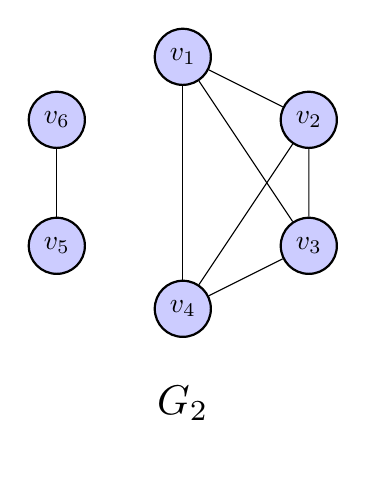
\begin{tikzpicture}
  [scale=.8,auto=left,every node/.style={circle,fill=blue!20,draw=black,thick}]
   \node (n1) at (2,4) {$v_1$};
  \node (n2) at (4,3)  {$v_2$};
  \node (n3) at (4,1)  {$v_3$};
  \node (n4) at (2,0) {$v_4$};
  \node (n5) at (0,1)  {$v_5$};
  \node (n6) at (0,3)  {$v_6$};

  \foreach \from/\to in {n1/n2,n2/n3,n1/n3, n1/n4, n2/n4, n3/n4,n5/n6}
    \draw (\from) -- (\to);

  % Etiqueta G_1 debajo del grafo
  \node[draw=none, fill=none, scale=1.5] at (2,-1.5) {$G_2$};

\end{tikzpicture}
